\documentclass[]{report}
\usepackage{graphicx, float}
\usepackage[export]{adjustbox}

\title{\centering CSL331 : First Assignment \\Part 1\\Booting in Windows and Linux}
\author{\LARGE Sahil\\2016UCS0008}

% to use proper section numbering in the report type 
\renewcommand{\thesection}{\arabic{section}}

\begin{document}

\maketitle

%%%%%%%%%%%%%%%%%%%%%%%%%%%%%%%%%%%%%%%%%%%%%%%%

\section{Booting in Windows (Reference version = Windows 10)}

\begin{figure}[H]
	\vspace{0pt}
	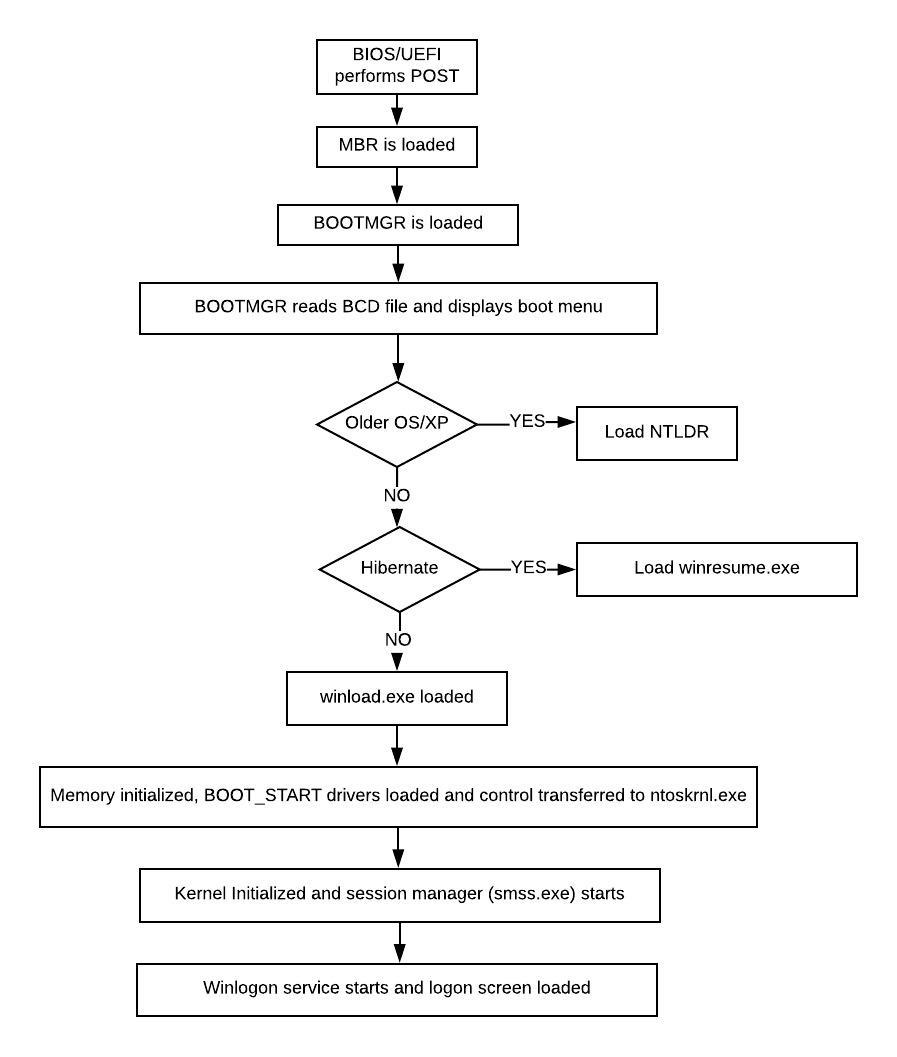
\includegraphics[height = 350pt, keepaspectratio]{windows_booting.jpeg}
\end{figure}


\large
\subsection{Step 1:} 
The UEFI or BIOS performs power-on-self-test (POST). During POST, quick tests are conducted and errors caused by incompatible hardware, disconnected devices, or failing components are displayed, with error messages such as "keyboard error or keyboard not present" or warnings. \\
The BIOS enables compter to access peripherals such as hard disks, keyboard, and the computer display prior to loading the OS.
\subsection{Step 2:}
The computer uses information in the UEFI or BIOS to locate an installed hard disk, which contains Master Boot Record (MBR) file on the first secgtor (512 bytes) of hard disk. MBR has information about the active portion on hard disk and from their computer calls and loads BOOTMGR.
\subsection{Step 3:}
BOOTMGR reads the BCD file from the active partition, gathers information about the machine's installed OSes, and then displays a boot menu, if the machine is in dual boot.
\subsection{Step 4:}
BOOTMGR either transfers control to winload.exe or calls winresume.exe if machine was hibernated. If winload.exe selects an earlier OS, such as Windows XP, then BOOTMGR transfers control to NTLDR.
\subsection{Step 5:}
Otherwise, winload.exe initializes memory and loads drivers that are set to begin at startup. These drivers are called BOOT\_START drivers and are for fundamental hardware components such as disk controllers and peripheral bus drivers. Winload.exe then transfers control to the OS kernel, ntoskrnl.exe.
\subsection{Step 6:}
The kernel initializes, and then higher-level drivers load (except BOOT\_START and services). During this phase, you will see the screen switch to graphical mode as the session manager (smss.exe) initializes the windows subsystem.
\subsection{Step 7:}
The windows OS loads the winlogon service, which displays the sign-in screen. Once the user signs in to the computer, windows explorer loads.

\section{Booting in Linux (Ubuntu)}

\begin{figure}[H]
	\vspace{0pt}
	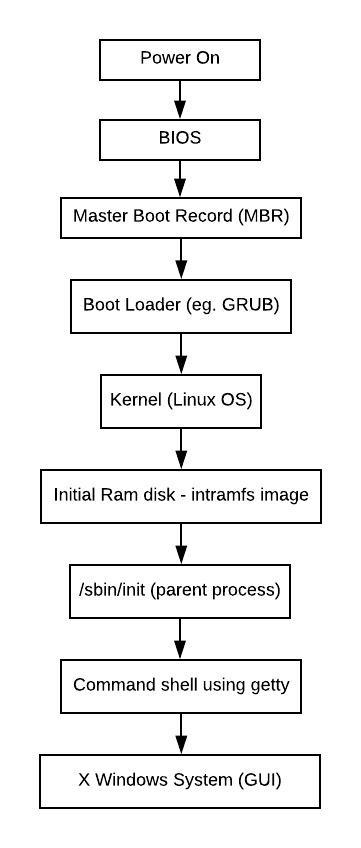
\includegraphics[height = 350pt, keepaspectratio]{linux_booting.jpeg}
\end{figure}


\large
There are 4 phases to starting up the system:
\begin{itemize}
	\item BIOS
	\item Boot Loader
	\item Kernel
	\item Upstart (which manages system tasks and services)
\end{itemize}
\subsection{BIOS phase:}
When the computer begins execution, it starts by executing this code, called as firmware, as it is normally stored in ROM, on the computer's motherboard. \\
This code must initialize the hardware other than the CPU, and obtain code for the next step, boot loader.
\subsection{Boot Loader phase:}
There are several possible types of boot loaders and ways for the BIOS to obtain them.
\begin{itemize}
	\item A boot loader stored in the first sector of a hard disk, the MBR. This may be GRUB or LILO.
	\item A boot loader stored on some other storage device, such as CDR or Flash Drive.
	\item A boot loader which uses the network, such as Pre-Execution environment.
\end{itemize}
The need for initial parts of the bootloader code on the first part of a storage medium explains why some hard drives are bootable and others are not. The job of the boot loader is to begin the next phase, loading the kernel and an initial ram disk filesystem.
\subsection{Kernal Phase:}
The kernel is the core code of an OS, providing access to hardware and other services. The bootloader starts the kernel running. To keep kernels to a reasonable size and permit separate modules for special hardware, modern kernels also use a file system which is present in memory, called an 'initrd' or 'initial ram disk'. The kernel launches the init script inside the initrd file system, which loads hardware drivers and finds the root partition.
\subsection{System Startup:}
After the kernel is running, the remainder of the OS is brought online. First, the root partition and the filesystem is located, checked and mounted. Next, the init process is started, which runs the initialization scripts. These scripts involve different /etc/rc scripts and upstart events that eventually gives you a ready-to-use computer with a login screen. 
\\
Some core boot tasks started by upstart are - 
\begin{itemize}
	\item Plymouth - The graphical boot animation and logger
	\item mountall - Mounts all filesystems obtained on /etc/fstab
	\item network - Network related services
	\item Display manager-  (GDM, KDM, XDM, ...)
\end{itemize}
\end{document}